\documentclass[a4paper, 12pt]{article}
\usepackage{graphicx}
\usepackage{subfig}
\usepackage{listings}
\usepackage{color}
\usepackage{amsfonts}
\graphicspath{ {./code/out/} }

\definecolor{dkgreen}{rgb}{0,0.6,0}
\definecolor{gray}{rgb}{0.5,0.5,0.5}
\definecolor{mauve}{rgb}{0.58,0,0.82}

\lstset{frame=tb,
  language=R,
  aboveskip=3mm,
  belowskip=3mm,
  showstringspaces=false,
  columns=flexible,
  basicstyle={\small\ttfamily},
  numbers=none,
  numberstyle=\tiny\color{gray},
  keywordstyle=\color{blue},
  commentstyle=\color{dkgreen},
  stringstyle=\color{mauve},
  breaklines=true,
  breakatwhitespace=true,
  tabsize=4
}

\begin{document}

    \pagenumbering{gobble}
    \begin{titlepage}
        \begin{center}

        \Large\textbf{Assignment}
         
        \large\textit{STAT 1003}

        \vspace{4cm}
        By Stephan Kashkarov

        u6729293
      \end{center}
      \vspace*{\stretch{2.0}}
    \end{titlepage}
    \tableofcontents
    \newpage
    \pagenumbering{arabic}

    \section{Question 1}
    \subsection{a}
        \renewcommand{\figurename}{Figure 1.a}
        \begin{figure}[h]
            \center{
                \subfloat[(i). Histogram of data w/ outliers]{
                    {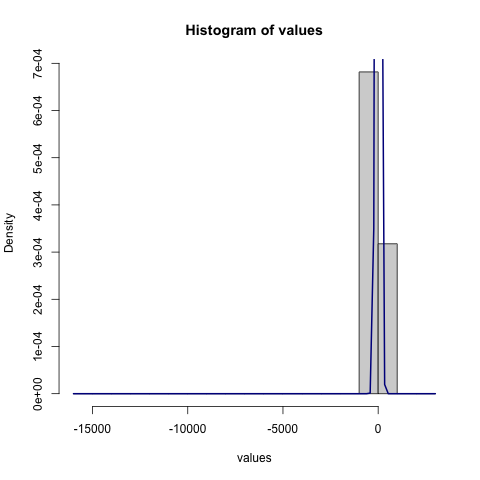
\includegraphics[width=5cm]{1.a.i.png} 
                }}%
                \qquad
                \subfloat[(ii). Histogram of data w/o outliers]{
                    {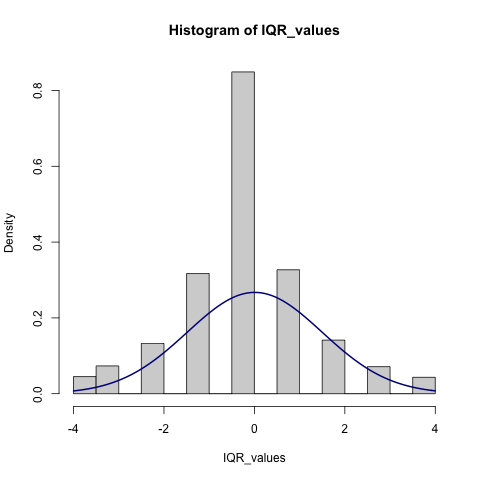
\includegraphics[width=5cm]{1.a.ii.png}
                }}%
                \qquad
                \subfloat[(iii). Normal Q-Q plot w/ outliers]{
                    {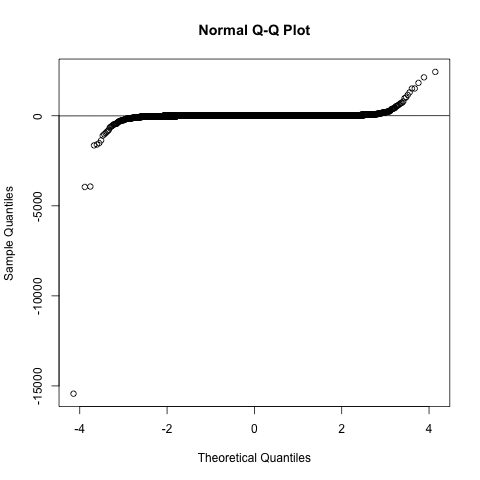
\includegraphics[width=5cm]{1.a.iii.png} 
                }}%
                \qquad
                \subfloat[(iv). Normal Q-Q plot w/o outliers]{
                    {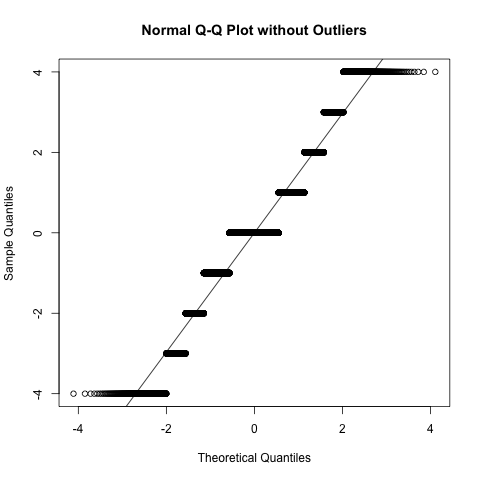
\includegraphics[width=5cm]{1.a.iv.png}
                }}%
            }
            \caption{}
            \label{fig:mesh1}
        \end{figure}
        According the the course material, the two ways to test for normality are: 
        \begin{itemize}
            \item Creating a frequency histogram and overlaying a curve
            \item Creating a Normal Q-Q plot
        \end{itemize}
        As seen in figure 1.a.i, the plot has a heavy outlier which makes it difficult to see the data. The data must be observed without the outliers to determine normality. This is seen in figure 1.a.ii

        The filtered data shows that there is a normal like structure in the data in the IQR of Q1 to Q3. This distribution looks to have lighter tails then the normal distribution with the same mean and sd.


        The normal Q-Q plot of the data, figure 1.a.iii, suffers the same issue as the histogram above. Figure 1.a.iv contains the data withing the IQR of Q1 and Q3 in a Q-Q plot.

        The IQR range QQ plot has a distinct stepping effect. The fact that the data is not continuous is the reason for this. Despite this we can see that the approximate middle of the the groups is along the line. A slight sinusoidal pattern can be seen in the data which reflects the data's lighter tails as observed above. 

    \subsection{b}
        The distribution shown in figures above seems to have lighter tails due to the symmetric pattern seen in the normal Q-Q plot. The histogram also supports the lighter tails hypothesis due to the large central grouping in the IQR plot. This central grouping shows that there is more values closer to the center hence lighter tails.

    \subsection{c}
        Apart from the obvious skew in figure 1.a.i, most of the indicators of the data point towards the symmetry of the distribution. To start with, the normal Q-Q plot with the outliers included seems to adhere to the line very symmetrically with the exception of the very large outlier. In the smaller

        Below find the code used to generate the related graphs:
        \lstinputlisting[language=r]{code/Q1.R}

    \pagebreak
    \section{Question 2}
    
    \subsection{a}
        \renewcommand{\figurename}{Figure 2.a}
        \begin{figure}[h]
            \centering
            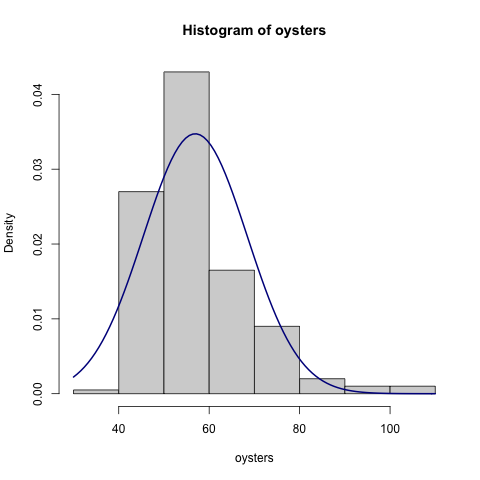
\includegraphics[width=0.8\textwidth]{2.a.i.png}
            \caption{(i) Histogram with normal curve overlay}
            \label{fig:mesh1}
        \end{figure}
        Figure 2.a.i contains an image of the histogram with an overlaid curve. From this figure we can see that the distribution does resemble a uni-modal normal distribution with a heavy right skew. 

    \subsection{b}
        \renewcommand{\figurename}{Figure 2.b}
        \begin{figure}[h]
            \centering
            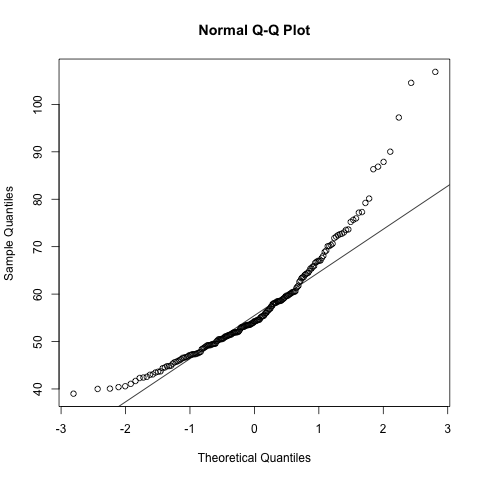
\includegraphics[width=0.8\textwidth]{2.b.i.png}
            \caption{(i) Histogram with normal curve overlay}
            \label{fig:mesh1}
        \end{figure}
        Using the two methods defined above we can check for normality. The first is already completed in figure 2.a.i. This figure shows a heavy right skew when compared to the blue ideal distribution but the distribution still looks normal. Figure 2.b.i contains an image of the normal Q-Q plot constructed from the data.  The QQ plot of the data shows how the normal distribution certainly does not fit perfectly. The line diverges from the curve around the 60th percentile and around the 45th percentile. The lower divergence is not as worrisome as it just shows the lighter tails of the data. The upper divergence shows that the data is heavily skewed on the right side of the distribution. This makes the distribution only just acceptable to be assumed to be normal.

        The code used to generate the two figures(2.a.i, 2.b.i) above shown below:
        \begin{lstlisting}
# Importing related data
oysters <- read.delim("data/oysters.txt", header = FALSE, sep=" ")
oysters <- stack(oysters)$values # converting block into column

# a.i - Creating a density histograph with curve line
png(filename="out/2.a.i.png") # outputs a png
hist(oysters, prob=T)
curve(dnorm(x, mean=mean(oysters), sd=sd(oysters)), col="darkblue", lwd=2, add=TRUE, yaxt="n")
dev.off() # resets display

# b.i - Creating a normal Q-Q plot of the data
png(filename="out/2.b.i.png") # outputs a png
qqnorm(oysters, main = "Normal Q-Q Plot")
qqline(oysters, datax = FALSE, distribution = qnorm)
dev.off() # resets display
        \end{lstlisting}

    \subsection{c}
        The distribution $\bar{X}$ can be defined by $\mu$ and $\sigma$ as such: 

        \[ \bar{X} \sim \mathcal{N} (\mu, \frac{\sigma^2}{n} ) \]

        where the expected value and variance of $\bar{X}$ can be defined as such:

        \[ \mathbb{E} (\bar{X}) = \mu \]
        \[ Var(\bar{X}) = \frac{\sigma^2}{n} \]

        since we do not know either proportion exactly we can use sample variables to calculate these values. $\mu$ can be calculated as 54.24 and $\sigma ^ 2$ can be calculated as 131.9338 which when substituted into the formula defined above yields:

        \[ \bar{X} \sim \mathcal{N} (54.24, \frac{131.9338}{200} )\]

        This is all assuming that the variables $\bar{X}$ and $S^2$ are relatively close to the true $\mu$ and $\sigma ^ 2$.
    \pagebreak

    \subsection{d}
        Below you will find the R code i used to calculate the 99\% confidence interval of the data.

        \begin{lstlisting}
# ... (continuing on from Q2.R)
# d.i - Calculating the 99% confidence interval.
n <- length(oysters)
m <- mean(oysters)
s <- var(oysters)
error <- qnorm(0.995)*s/sqrt(n)
lowerBound <- m-error
upperBound <- m+error
cat("99% confidence interval is (" , lowerBound , "," , upperBound, ")\n")
#[1] 99% confidence interval is ( 32.89357 , 80.95406 )
        \end{lstlisting}
        In the code above, n, m and s represent the sample size, the mean and the standard deviation respectively. These are drawn from the values defined in Q2.c. These values are then used to shift a qnorm of 0.995. the decimal value in this is halve of 1\% to ensure that both tails add up to 1\%. The error is then subtracted and added to the mean to calculate lower and upper tails. This is then printed with a function called cat to give us the interval of $(32.89357, 80.95406)$. This is all done assuming that the oysters fall into a normal distribution

    \subsection{e}
        There are countless ways that the sample could be invalidated. For example the sample could have been taken at a very high/low yield time of the year. This would not represent the number of oysters as $\bar{X}$ would nor work properly in other times of the year. This could be avoided by sampling from all times in the year. They could have all been taken from one part of the farm where they where easily accessible which would also skew the data. There are many ways which skew could be introduced into the data.
    \pagebreak
    \section{Question 3}
    \subsection{b}
    \lstinputlisting[language=r]{code/Q3.R} 
    \section{Question 4}
    \subsection{a}
        To formulate a test for the described criteria the following must be done. As this is a paired sample and sd is assumed equal, we subtract each value in the male category by each value in the female. However since they are not equal in length we can simply subtract the two means $\bar{X}$ $\bar{Y}$ to get us a new mean $\bar{W}$. $S^2$ also has to be calculated differently \[{S^2}_d = \frac{1} {n}(\sum (x_i - y_i - n\bar{W}^2))\] From there we can run the test as usual. We assume that all elements in X and Y are iid normal variables.

    \subsection{b}
        The test statistic for the above test would be as follows
        \[ T = \frac {\bar{W}} {{S^2}_d / \sqrt{n} }\] which is of distribution $\mathcal{T}_{n-1}$

    \subsection{c}
    I was unaware this assignment was due at 5 instead of 12. I had to run home from work haha

\end{document}